\section{Objectives}

Manipulation of objects is one of the most natural action of humankind. Humans never stood and planned about how to manipulate an item. It is an instinct for humans to grab objects in specific ways. Even an infant human can easily manipulate different shapes and colors of objects. Manipulation helps us to use tools, gadgets and provide services. From rehabilitation to service robots, tool usage is vital to enable them to achieve their objective.
Therefore, manipulation skills will be central for robots of any kind. 
Example of our daily manipulation tasks are shown in figure \ref{fig:x manipulation_skills}.

For a complicated manipulation task, first of all, grasping the object is essential. We need first firmly to grab a water bottle to drink it.
Without a firm grasp, the manipulation process will not be safe. 
Nowadays, every kind of robot is helping us produce in the industry. The task robots are responsible for expands from the car manufacturing to high precision microchip producing. On all those tasks, robots are incredibly efficient and precise. However, these tasks' common denominator is that they are repetitive and specialized in a specific process. If a car company decides to manufacture a new car model, the whole process may need to be changed, and the robot's program needs to be hardcoded from zero. Eventually, we want to avoid this redundant task of programming all from zero each time we change the process.

This master's thesis's main objective is to enable robotic 
manipulators to incrementally learn to grasp tools and generalize the learned policy to unseen objects. This procedure promises a robust gripper that can adapt well to unseen objects and environments.. Moreover, rather than hardcoding robot's every move, we take another approach, that the robot learns by itself based on the observation and rewards it receives from the simulation environment. We vision that through learning-based methods, robots will learn to extrapolate their knowledge to unknown objects and processes \ref{fig:graspseq}.

\begin{figure}[htbp]
    \centering
      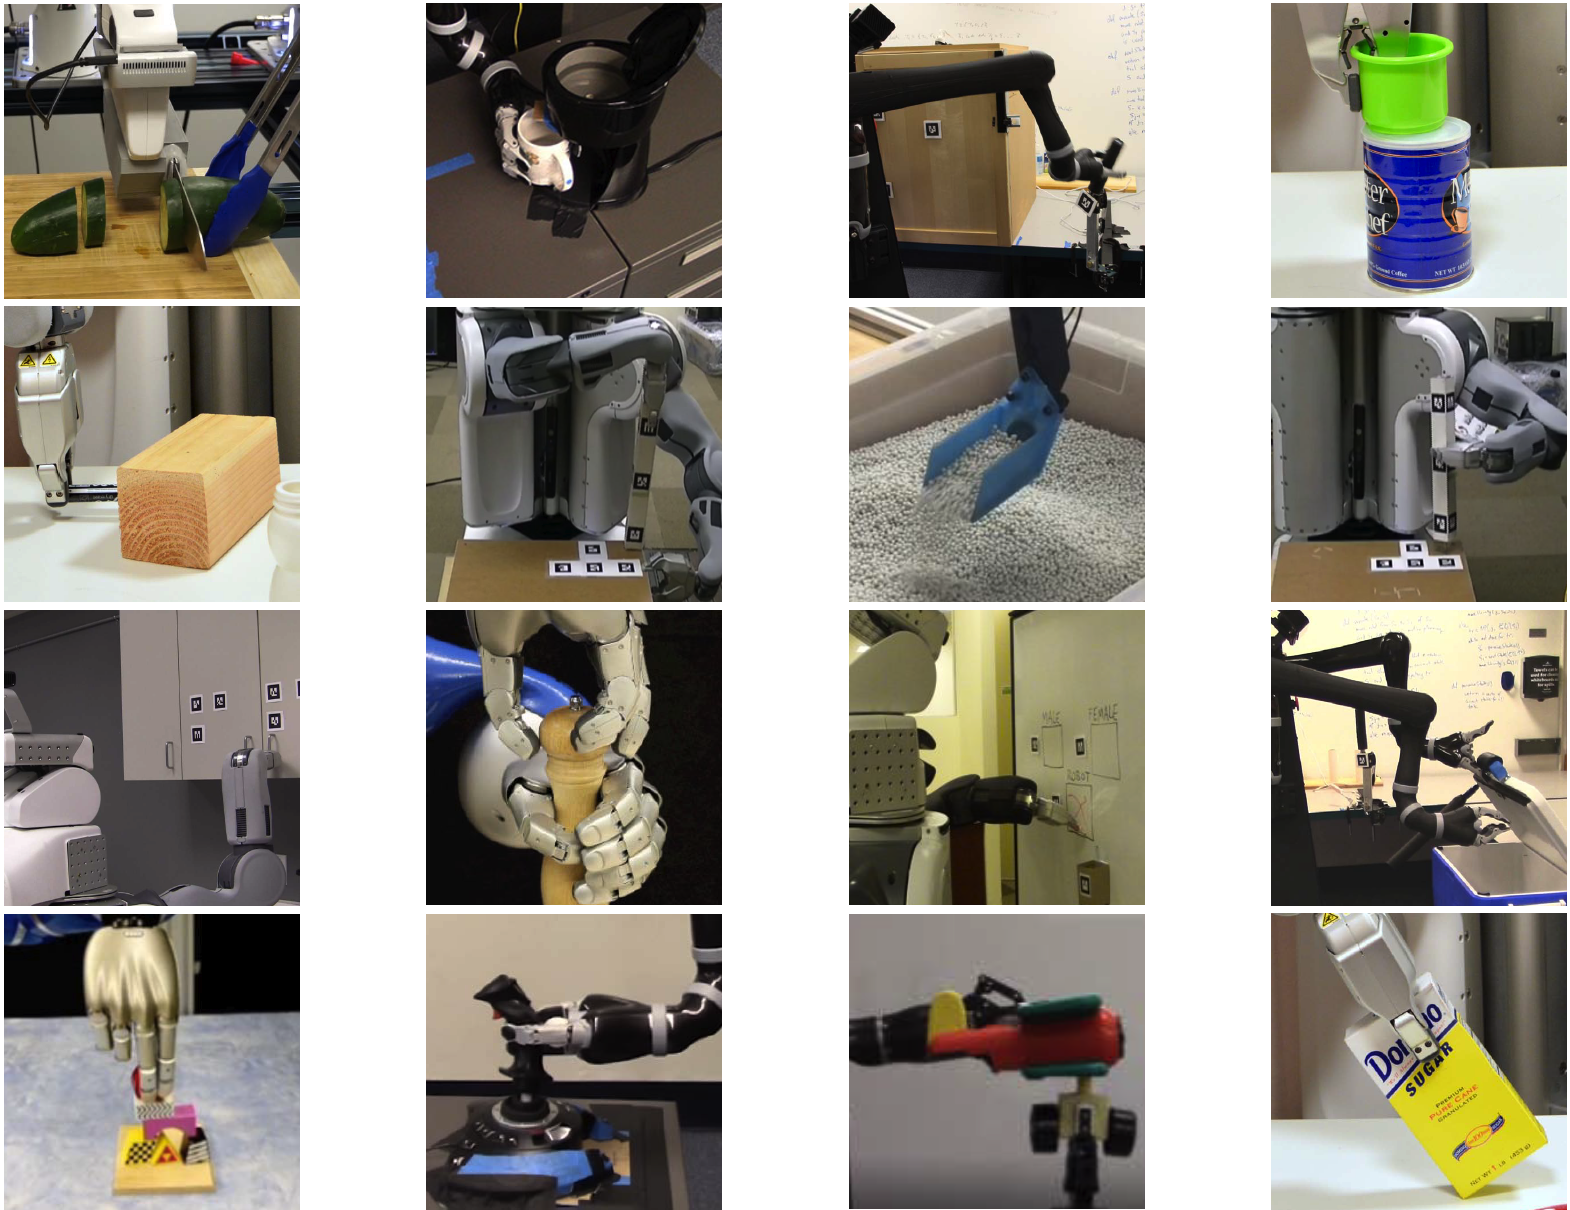
\includegraphics[width=0.8\textwidth]{figures/manipulation_skill}
    \caption{Different manipulation skill adopted to robotic manipulators \cite{Kroemer2019}}
    \label{fig:x manipulation_skills}
\end{figure}

% \begin{figure}[!htbp]
%   \begin{subfigure}{0.49\textwidth}
%       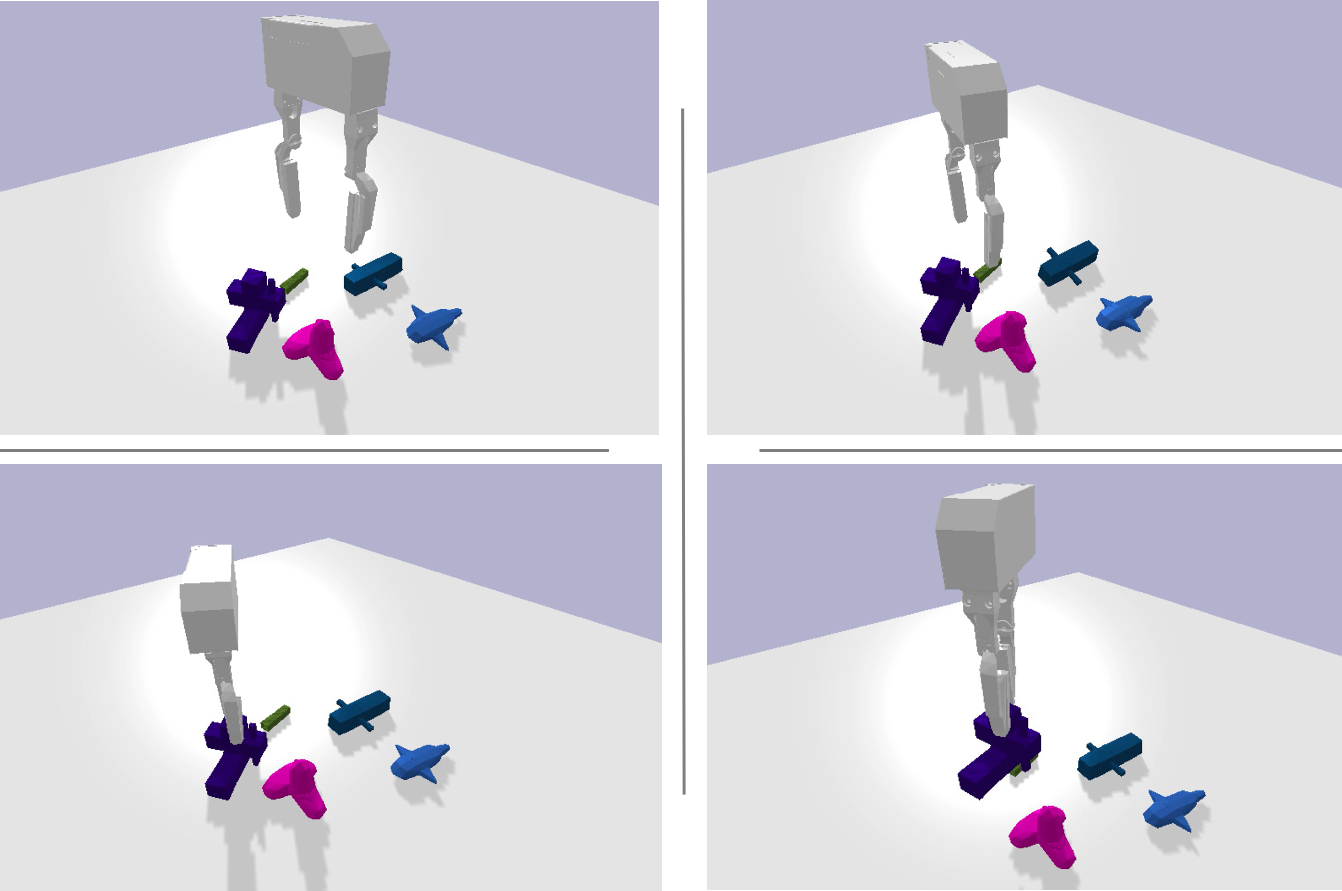
\includegraphics[width=\linewidth]{figures/newfloor}
%       \caption{Grasp sequence in floor scene} \label{fig:table}
%   \end{subfigure}%
%   \hspace*{\fill}   % maximize separation between the subfigures
%   \begin{subfigure}{0.49\textwidth}
%       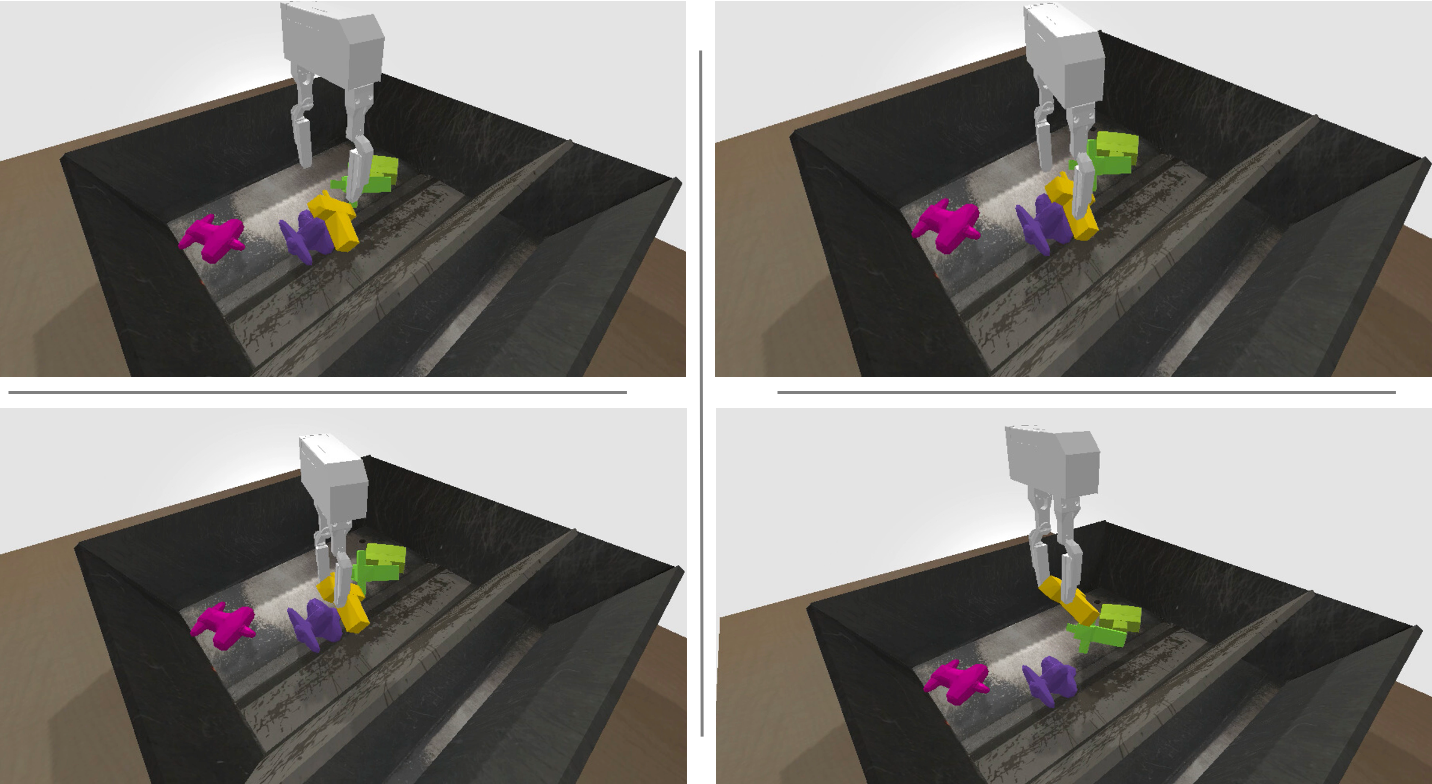
\includegraphics[width=\linewidth]{figures/newtable}
%       \caption{Grasp sequence in table scene} \label{fig:floor}
%   \end{subfigure}%
%   \hspace*{\fill}   % maximize separation between the subfigures    
%   \caption{ Our robot model performs grasping on floor and table scene\label{fig:graspseq}}
% \end{figure}



\begin{figure}[htbp]
  \centering
    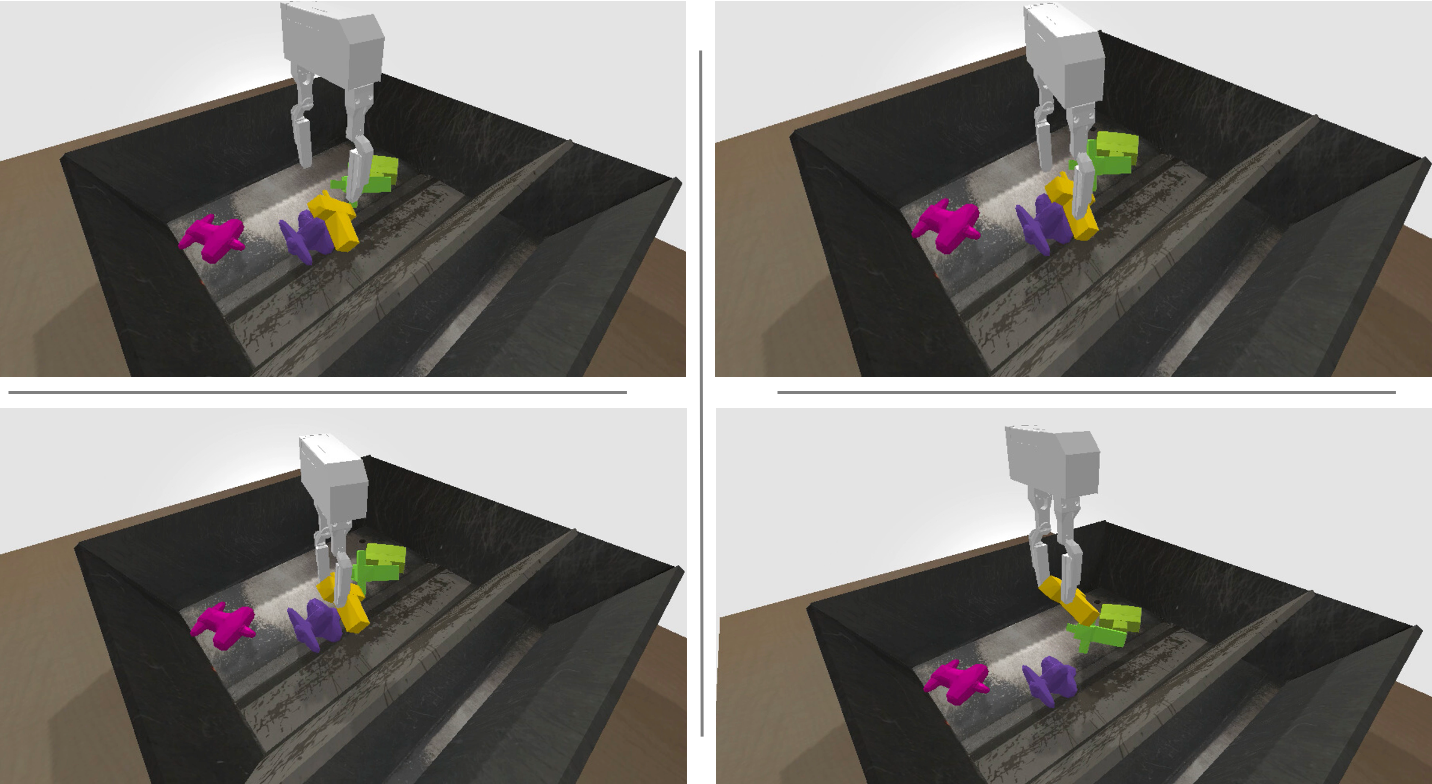
\includegraphics[width=1.\textwidth]{figures/newtable}
  % \caption{Different manipulation skill adopted to robotic manipulators \cite{Kroemer2019}}
  % \label{fig:x manipulation_skills}
  \caption{ Our robot model performs grasping on floor and table scene\label{fig:graspseq}}
\end{figure}

% \begin{figure}[htbp]
%   \centering
%     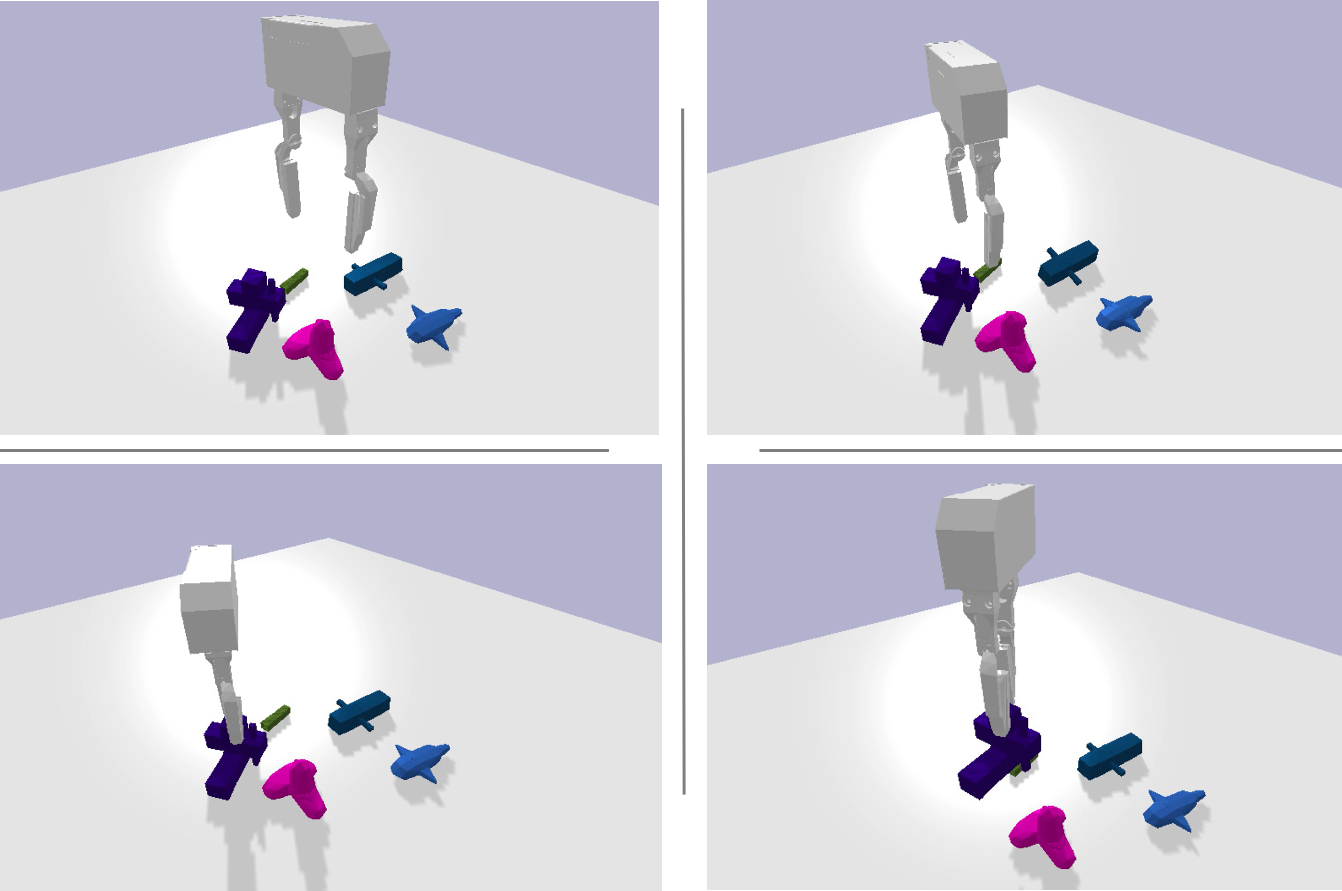
\includegraphics[width=1.\textwidth]{figures/newfloor}
%   \caption{Different manipulation skill adopted to robotic manipulators \cite{Kroemer2019}}
%   \label{fig:x manipulation_skills}
% \end{figure}